\documentclass[12pt]{article}

\usepackage[a4paper,margin=1in]{geometry}
\usepackage[utf8]{inputenc}
\usepackage[spanish,es-tabla]{babel}
\usepackage{graphicx}
\usepackage{circuitikz}
\usepackage{amsmath}
\usepackage{subcaption}
\usepackage{amssymb}
\usepackage[hidelinks]{hyperref}
\usepackage{mathtools}
\usepackage{enumitem}
\usepackage{array}
\usepackage{longtable}
\usepackage{multirow}
\usepackage{csquotes}
\usepackage{float}
\usepackage{setspace}
\usepackage{pdflscape}
\usepackage{pgfplots}
\pgfplotsset{compat=1.18}
\usetikzlibrary{arrows.meta, decorations.pathreplacing, calc, positioning}
\usepackage[style=ieee, backend=bibtex]{biblatex}
\addbibresource{bibliografia.bib}
\graphicspath{{Figuras/}{Planos/}}
\onehalfspacing

\hypersetup{
    colorlinks=true,
    linkcolor=blue,
    citecolor=blue,
    urlcolor=blue,
    filecolor=blue
}

% Marca en rojo lo que falta completar. Para la entrega, buscar "\pendiente" y verificar que no quede ninguno.
\newcommand{\pendiente}[1]{\textcolor{red}{\textit{[Pendiente: #1]}}}

\begin{document}
\renewcommand{\figureautorefname}{Fig.}
\renewcommand{\tableautorefname}{Tab.}
\renewcommand{\equationautorefname}{Ec.}

\begin{titlepage}
\thispagestyle{empty}
\begin{tikzpicture}[remember picture,overlay]
    \node[opacity=0.2,anchor=center] at (current page.center)
        {
\includegraphics[width=0.9\paperwidth]{decoracion_a.png}};
\end{tikzpicture}
\begin{center}
    
\includegraphics[width=15cm]{unc_fcefyn_logo.png} \\ [0.5cm]
    \LARGE Universidad Nacional de Córdoba \\ [0.5cm]
    \large Facultad de Ciencias Exactas, Físicas y Naturales \\
    \vspace{40pt}
    \large Sistemas de Radiocomunicación \\ [0.2cm]
    \large Trabajo Práctico N°4: Parte 2\\
    \vspace{60pt}
    \LARGE Diseño de una Red FTTH con Tecnología GPON\\[0.3cm]
    \large Marcos Juárez, Córdoba\\
    \vspace{50pt}
    \begin{table}[!h]
        \centering
        \begin{tabular}{ll}
            \multicolumn{1}{c}{Nombre} & \multicolumn{1}{c}{DNI} \\
            Arteaga Barrera, Cristian Eduardo   & 95.159.096 \\
            Baccino, Luca                       & 45.328.380 \\
            Mendes Rosa, Agustín                & 44.517.201 \\
            Monja, Ernesto Joaquín              & 43.873.728
        \end{tabular}
    \end{table}
    \vspace{20pt}
    \begin{table}[!h]
        \centering
        \begin{tabular}{ll}
            \multicolumn{1}{c}{Docentes} & Esp. Ing. Liendo, Carlos Guillermo \\
                                         & Ing. Dadam, Federico Tomás \\
        \end{tabular}
    \end{table}
    \vfill
        {\small Córdoba, República Argentina\\
                Año 2026}
\end{center}
\end{titlepage}
\newpage

\tableofcontents
\newpage
\listoffigures
\newpage
\listoftables
\newpage

% Un archivo por cada punto de la consigna
\section{Introducción}
\label{sec:introduccion}
La fibra óptica constituye un medio fundamental para las redes de telecomunicaciones: se utiliza en enlaces de transporte, en conexiones punto a punto y en redes de acceso FTTH (\textit{Fiber to the Home}, fibra hasta el hogar). Las redes FTTH con tecnología GPON permiten brindar acceso a Internet, telefonía, televisión y otros servicios mediante una infraestructura óptica compartida, cuyo diseño requiere integrar criterios de cobertura, capacidad, distribución de fibras, selección de componentes y presupuesto óptico.

En este trabajo se desarrolla una propuesta de red FTTH GPON para la localidad de Marcos Juárez, provincia de Córdoba, tomando como referencia el área de cobertura indicada por la cátedra (\autoref{fig:area_cobertura}). El nodo cabecera se ubica en la Cooperativa COYSPU (9 de Julio 99-149) y el área se divide en las regiones Este y Oeste según la traza de la Ruta Nacional 12.

\begin{figure}[H]
    \centering
    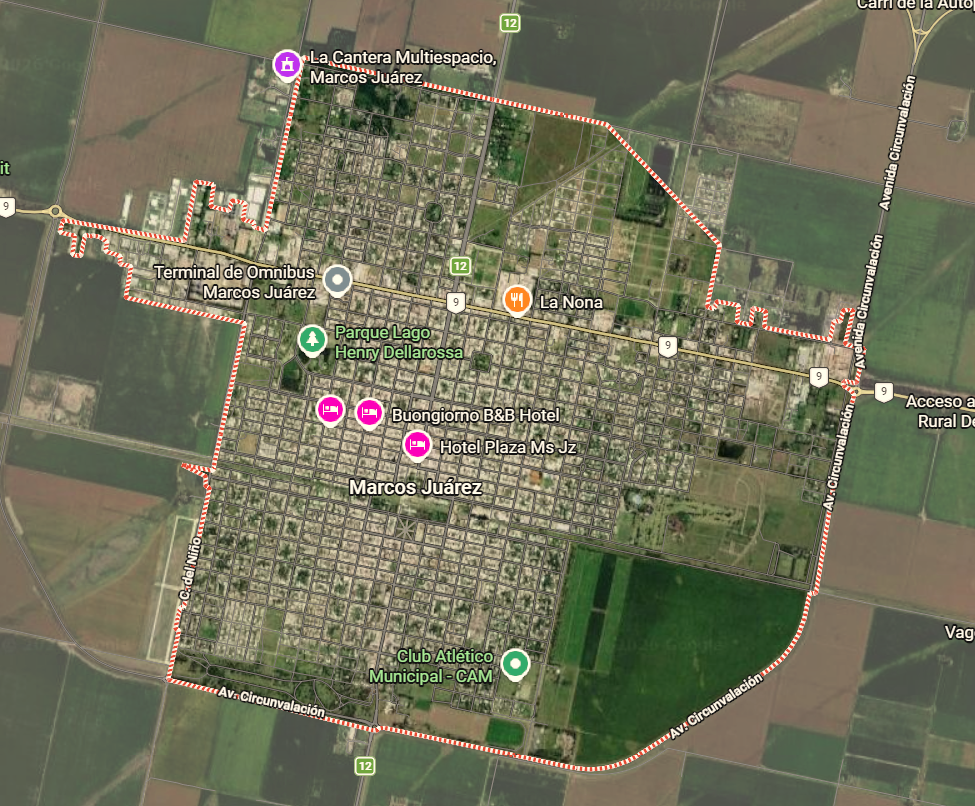
\includegraphics[width=0.85\textwidth]{area_cobertura.png}
    \caption{Área de cobertura de la red en la localidad de Marcos Juárez. Fuente: consigna de la cátedra.}
    \label{fig:area_cobertura}
\end{figure}

\pendiente{describir la organización del informe una vez completadas las secciones.}



\section{Investigación sobre infraestructura óptica y servicios}
\label{sec:investigacion}

\subsection{REFEFO y ARSAT}
\label{sec:refefo}
% Consigna 1.1:
% - Significado de la sigla y objetivos de la red.
% - Desarrollo, cobertura y servicios que ofrece.
% - Función de la REFEFO como infraestructura de transporte y conectividad mayorista.
% - Relación con los operadores que brindan servicios de acceso a los usuarios.
% - Actividades de ARSAT vinculadas con fibra óptica, televisión digital y servicios satelitales.
% - Indicar fuentes y FECHA DE CONSULTA.
% Fuente útil: material de cátedra, "Libro Cap 1 a 5 parte II", sección 1.7.
\pendiente{síntesis sobre la REFEFO y ARSAT, con fuentes y fecha de consulta.}

\subsection{Fundamentos de fibra óptica}
\label{sec:fundamentos}
% Consigna 1.2: síntesis integrada de los 5 videos indicados por la cátedra y
% explicación de qué conceptos son relevantes para el diseño FTTH y la selección de componentes.
\pendiente{síntesis integrada de los videos y su relevancia para el diseño FTTH.}

\subsection{Cables submarinos}
\label{sec:submarinos}
% Consigna 1.3: mapa de cables submarinos con llegada a Las Toninas.
% - Sistemas representados, destinos principales y estado informado.
% - Función en la conectividad internacional de Argentina y relación con las redes terrestres.
% Fuente útil: material de cátedra, "Libro Cap 1 a 5 parte II", sección 1.8.
\pendiente{sistemas que llegan a Las Toninas, destinos, estado y su rol en la conectividad.}

\newpage


\section{Análisis de catálogos y selección de componentes}
\label{sec:componentes}
% Fuentes iniciales sugeridas: Furukawa/Lightera, Huawei, VSOL, KOC, Wiretech (Córdoba).
% Se pueden usar otros fabricantes, incorporando las fichas técnicas y la fuente.

\subsection{Cables ópticos}
\label{sec:cables}
% Consigna 2.1: comparar cables para troncal/alimentación, distribución y acceso al abonado;
% tendido aéreo, por ductos o directamente enterrado.
% Para cada alternativa relevar: tipo de fibra y norma, cantidad de fibras y organización interna,
% atenuación por longitud de onda, construcción y protección, radio mínimo de curvatura,
% tracción máxima y demás parámetros mecánicos.
% Explicar qué cable se usa en cada tramo y justificar.
\pendiente{tabla comparativa de cables por tramo y justificación de la elección.}

\subsection{Componentes pasivos y equipos activos}
\label{sec:pasivos_activos}
% Consigna 2.2: cajas de empalme y cierres, cajas de distribución y terminales de acceso (NAP),
% splitters, conectores/adaptadores/pigtails/patch cords, distribuidores ópticos (ODF),
% OLT y ONU/ONT (los activos deben ser GPON).
% Presentar una tabla con: fabricante, modelo, función, especificaciones relevantes y aplicación prevista.
\pendiente{tabla de componentes pasivos y equipos activos GPON seleccionados.}

\newpage


\section{Reconocimiento de elementos en laboratorio}
\label{sec:laboratorio}
La \autoref{tab:laboratorio} relaciona los elementos disponibles en el laboratorio con su función, su ubicación dentro de la red diseñada y los componentes seleccionados en la \autoref{sec:componentes}.

\begin{longtable}{|p{2.4cm}|p{3.5cm}|p{3.2cm}|p{4.6cm}|}
    \caption{Elementos del laboratorio, su función y su ubicación en la red.}\label{tab:laboratorio}\\
    \hline
    \textbf{Elemento} & \textbf{Función} & \textbf{Ubicación en la red} & \textbf{Instalación y manipulación} \\
    \hline
    \endfirsthead
    \hline
    \textbf{Elemento} & \textbf{Función} & \textbf{Ubicación en la red} & \textbf{Instalación y manipulación} \\
    \hline
    \endhead
    Cable troncal de tubos holgados & Transportar las fibras desde el hub hasta los clusters & Postes, desde el hub hasta las CEO de cluster & Respetar el radio de curvatura ($20 \times D$ durante el tendido) y la tracción máxima; dejar rulos de reserva en las cajas \\
    \hline
    Cable de distribución (tubo central) & Llevar las fibras de la caja de distribución a las CTO & Postes dentro de cada sector & Abrir el tubo solo en la ventana de la caja (sangría) sin dañar las fibras que siguen de paso \\
    \hline
    Cable drop & Conectar la CTO con la vivienda & Entre el poste de la CTO y la fachada & Retirar el mensajero de acero solo en los extremos; fibra G.657.A, tolera curvaturas cerradas \\
    \hline
    Conectores y adaptadores SC/APC & Unión desmontable entre fibras & ODF, CTO, roseta y ONT & Inspeccionar y limpiar la férula antes de cada conexión; no mezclar APC (verde) con UPC (azul) \\
    \hline
    Pigtails y patch cords & Terminar fibras en paneles y conectar equipos & ODF del hub y domicilio & Empalmar los pigtails por fusión; no exceder el radio de curvatura en los organizadores \\
    \hline
    Splitter PLC & Dividir la potencia óptica entre varias salidas & Caja de distribución (1:4) y CTO (1:16) & Su pérdida aumenta con la relación de división (aprox. $10 \log N$ más la pérdida en exceso) \\
    \hline
    Caja de empalme (CEO) & Proteger empalmes y derivaciones & Derivaciones del troncal y cajas de distribución & Cierre hermético; ordenar las fibras en bandejas y respetar el radio mínimo de $30 \, [mm]$ \\
    \hline
    Caja terminal (CTO/NAP) & Punto de conexión de los drops & Postes, una por cada grupo de hasta 17 viviendas & Identificar cada salida; sellar los pasacables no utilizados \\
    \hline
    Empalmadora por fusión & Unir fibras con baja pérdida & Todas las cajas de empalme & Pelado, limpieza con alcohol isopropílico y corte con cortadora de precisión; descartar los restos de fibra en un recipiente \\
    \hline
    Localizador visual de fallas (VFL) & Verificar continuidad e identificar fibras & Mantenimiento y puesta en servicio & No mirar directamente el haz \\
    \hline
    Medidor de potencia óptica & Medir la potencia recibida & Puesta en servicio: salida de la CTO y roseta & Seleccionar la longitud de onda de calibración que corresponde a la señal medida \\
    \hline
    Peladora y cortadora de precisión & Retirar los recubrimientos y obtener un corte plano de la fibra & Preparación de todo empalme o conector & Respetar las longitudes de pelado y corte del accesorio; limpiar con alcohol isopropílico antes de cortar \\
    \hline
    Conector y empalme mecánicos & Terminar o unir fibras en campo sin empalmadora & Reparaciones de emergencia y acometidas & Empalme 3M Fibrlok II con herramienta 2501; insertar la fibra hasta formar el arco de control y proteger el empalme \\
    \hline
\end{longtable}

\subsection{Prácticas realizadas}
\label{sec:practicas_lab}
Las prácticas indicadas por la cátedra se realizaron con las herramientas de instalación del laboratorio, y su desarrollo completo se presenta en la Parte 2 del Trabajo Práctico N.° 3 \cite{informe_tp3}. A continuación se resumen los resultados y su relación con la red diseñada.

\textbf{Práctico A, detección visual de fallas:} se acopló el VFL a un tramo de cable y la luz roja apareció como un punto definido en el extremo opuesto, lo que confirmó la continuidad del hilo (\autoref{fig:lab_vfl}). Al medir esa luz con el medidor de potencia se obtuvo un valor distinto de cero pero no confiable, porque el VFL emite en $650 \, [nm]$ y la menor longitud de onda seleccionable en el medidor era $800 \, [nm]$: la respuesta del fotodetector depende de $\lambda$, y fuera de la longitud de onda de calibración la lectura solo indica presencia de señal.

\begin{figure}[H]
    \centering
    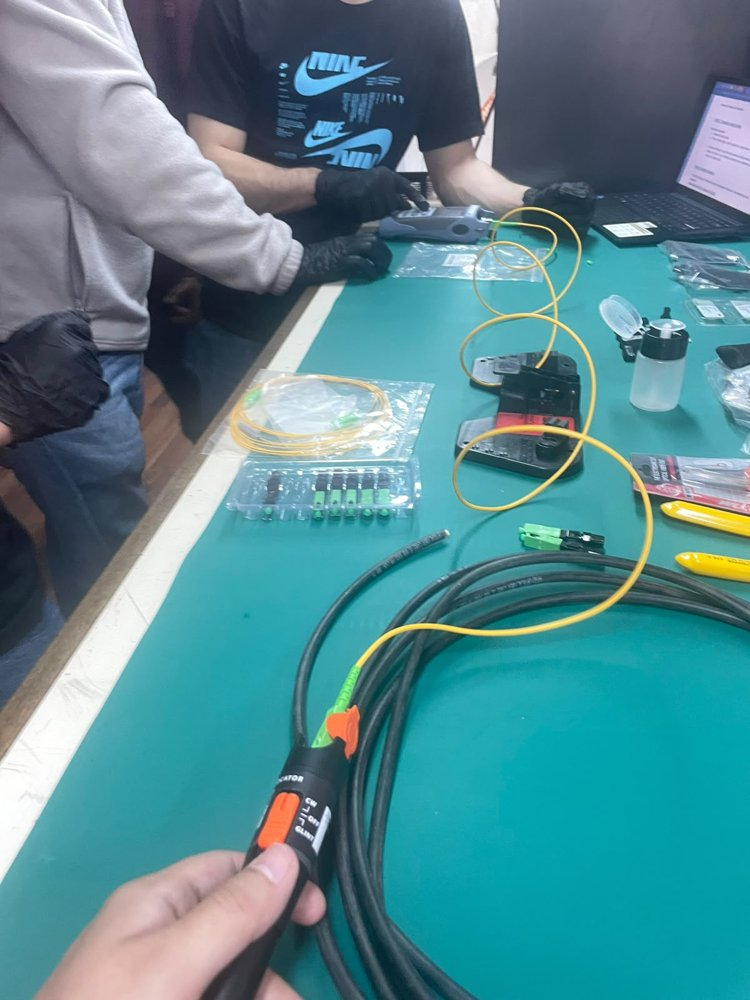
\includegraphics[width=0.28\textwidth]{lab_vfl_continuidad.jpg}
    \caption{Verificación de continuidad con el VFL y el medidor de potencia. Fuente: Trabajo Práctico N.° 3 \cite{informe_tp3}.}
    \label{fig:lab_vfl}
\end{figure}

\textbf{Práctico B, conectorización mecánica SC/APC:} se peló el cable, se limpió la fibra, se cortó a $10 \, [mm]$ con la cortadora de precisión y se insertó en el conector hasta formar el arco de control, que indica contacto contra el tope interno (\autoref{fig:lab_conector}). Se necesitaron varios intentos porque la fibra se quebraba durante la preparación. El conector quedó armado, pero el medidor de potencia no registró señal.

\begin{figure}[H]
    \centering
    \begin{subfigure}{0.22\textwidth}
        \centering
        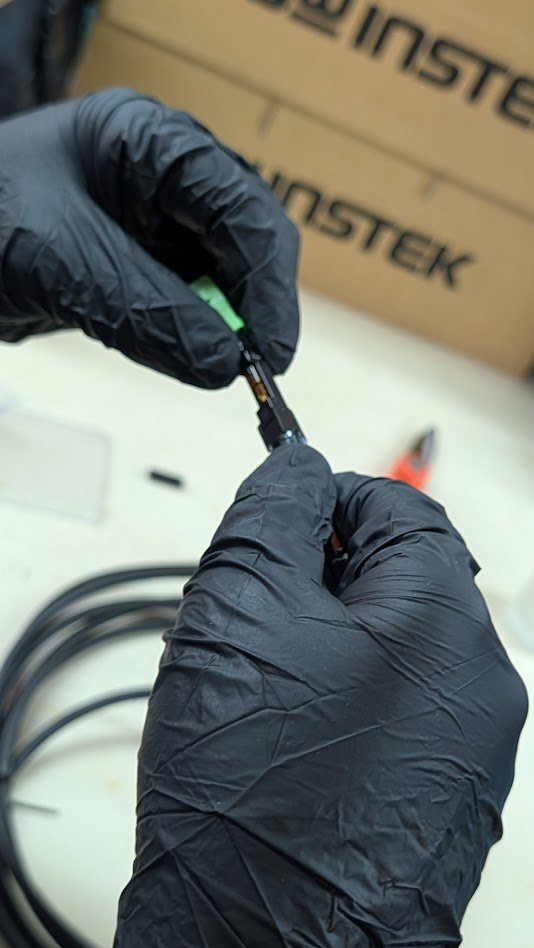
\includegraphics[width=\linewidth]{lab_conector_insercion.jpg}
        \caption{Inserción de la fibra cortada.}
    \end{subfigure}
    \hspace{1cm}
    \begin{subfigure}{0.30\textwidth}
        \centering
        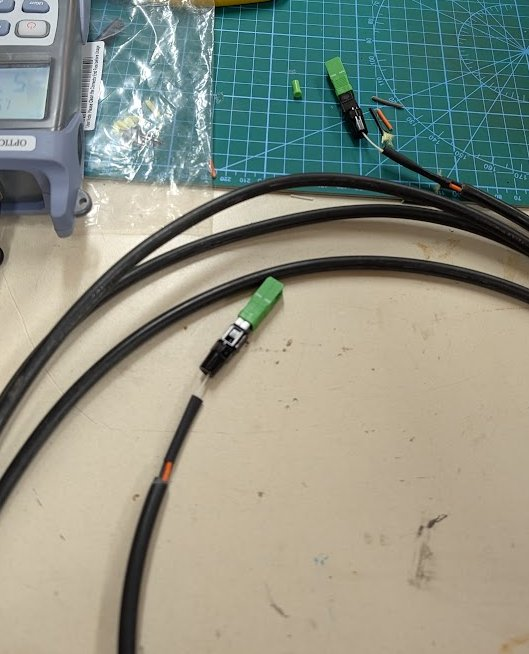
\includegraphics[width=\linewidth]{lab_conector_sc_apc.jpg}
        \caption{Conector SC/APC armado.}
    \end{subfigure}
    \caption{Montaje del conector mecánico SC/APC. Fuente: Trabajo Práctico N.° 3 \cite{informe_tp3}.}
    \label{fig:lab_conector}
\end{figure}

\textbf{Práctico C, empalme mecánico:} con la herramienta 3M 2501 se prepararon dos fibras (pelado, limpieza y corte a $12{,}5 \, [mm]$), se insertaron en el módulo de empalme hasta igualar los arcos y se cerró la tapa, que fija la alineación con gel adaptador de índice. Luego se colocó un protector sobre el empalme (\autoref{fig:lab_empalme}). Como se usó el mismo cable del práctico anterior, el medidor tampoco registró potencia. La falla se atribuyó a una rotura de la fibra en un punto del cable que no pudo ubicarse con el VFL, porque las capas de cubierta impedían ver la fuga de luz.

\begin{figure}[H]
    \centering
    \begin{subfigure}{0.30\textwidth}
        \centering
        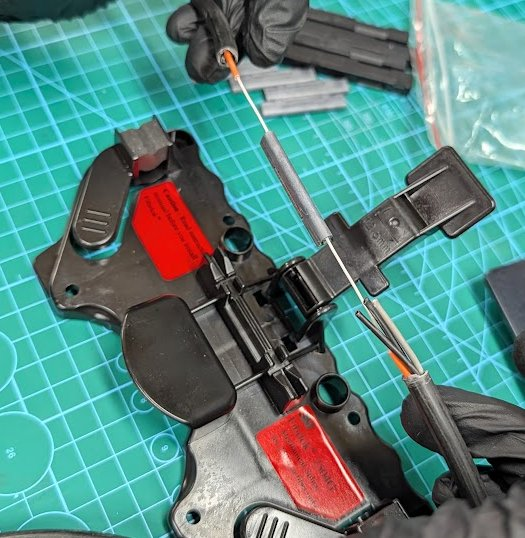
\includegraphics[width=\linewidth]{lab_empalme_mecanico.jpg}
        \caption{Empalme terminado.}
    \end{subfigure}
    \hfill
    \begin{subfigure}{0.62\textwidth}
        \centering
        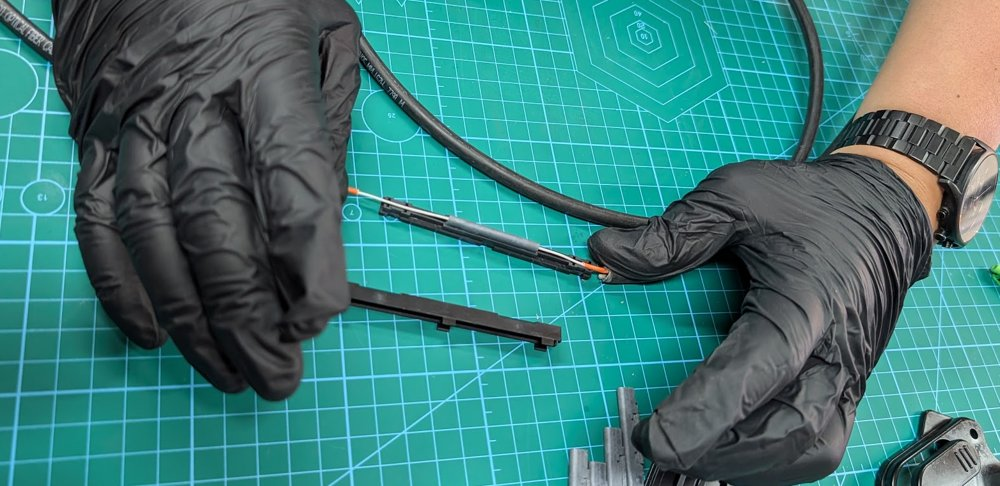
\includegraphics[width=\linewidth]{lab_empalme_protector.jpg}
        \caption{Colocación del protector.}
    \end{subfigure}
    \caption{Ejecución del empalme mecánico. Fuente: Trabajo Práctico N.° 3 \cite{informe_tp3}.}
    \label{fig:lab_empalme}
\end{figure}

\subsection{Vínculo con la Actividad N.° 3 y con el diseño}
En la Parte 1 de la Actividad N.° 3 se comprobó que la potencia que llega al receptor disminuye con la longitud de la fibra y con los acoplamientos imperfectos (al enfrentar los conectores a mano la señal se escuchaba más débil), y que el receptor digital deja de recuperar la señal cuando esta no supera su umbral \cite{informe_tp3}. En una red GPON el mismo principio se cuantifica con el presupuesto óptico: los splitters, conectores y empalmes reconocidos en el laboratorio son los eventos de pérdida que se suman en la \autoref{sec:presupuesto}, y la sensibilidad de la ONT y de la OLT cumple el papel del umbral de decisión.

Las prácticas de instalación respaldan las siguientes decisiones del diseño:
\begin{itemize}
    \item \underline{Empalmes por fusión en la planta externa:} la fragilidad observada al preparar la fibra a mano, y la falla que dejó el enlace sin señal, muestran que la calidad depende del operador. Un empalme mecánico bien ejecutado tiene una pérdida típica menor a $0{,}1 \, [dB]$, pero su reflectancia puede llegar a $-35 \, [dB]$ en todo el rango de temperatura \cite{fibrlok}, mientras que la fusión no tiene interfaz de gel y es permanente. Por eso el diseño adopta empalmes por fusión en las CEO, las cajas de distribución, la entrada de las CTO y la roseta, y reserva los empalmes mecánicos para reparaciones de emergencia. En el extremo del drop que se conecta a la salida SC/APC de la CTO se recomienda usar drops preconectorizados de fábrica; si se usan conectores mecánicos de campo como el del práctico B, cada acometida debe verificarse con el medidor de potencia al instalarla.
    \item \underline{Margen de ingeniería y reservas de cable:} cada reparación agrega empalmes, y en el laboratorio fueron necesarios varios intentos para obtener un corte correcto. El margen de $3 \, [dB]$ y los rulos de reserva de $20 \, [m]$ por caja de empalme y $10 \, [m]$ por CTO (\autoref{sec:trazas}) permiten rehacer empalmes sin reemplazar el cable.
    \item \underline{Instrumental de puesta en servicio:} el medidor de potencia debe estar calibrado en las longitudes de onda de la red ($1310$, $1490$ y, con video overlay, $1550 \, [nm]$), ya que fuera de ellas la lectura no es válida. El VFL sirve para verificar continuidad e identificar fibras en las cajas, pero no localiza roturas dentro de cables con cubierta: para eso se requiere un reflectómetro (OTDR), con el que deben certificarse los tramos al construir la red.
\end{itemize}

\newpage


\section{Alcance y etapas del proyecto}
\label{sec:alcance}
% Consigna 4. Requisito general: la infraestructura debe poder atender al 90 % de las viviendas,
% con 45 % en el primer año. Cuando no haya datos reales, formular supuestos explícitos y justificados.

\subsection{Área de cobertura y regiones de diseño}
\label{sec:area}
% 1. Delimitar el área de cobertura según la imagen de la consigna (Fig. area_cobertura).
% 2. Regiones Este y Oeste, divididas por la traza de la Ruta 12 (norte-sur).
\pendiente{delimitación del área y división en Región Este y Región Oeste.}

\subsection{Casas pasadas y abonados}
\label{sec:abonados}
% 3. Cantidad de casas pasadas.
% 4. Abonados estimados en la primera etapa y justificación del supuesto de adopción.
\pendiente{conteo de casas pasadas y abonados de la primera etapa (45 \%) y final (90 \%).}

\subsection{Servicios y planes de velocidad}
\label{sec:servicios}
% 5. Servicios y planes de velocidad considerados.
\pendiente{servicios ofrecidos y planes de velocidad.}

\subsection{Criterios de crecimiento y reserva}
\label{sec:crecimiento}
% 6. Criterios de crecimiento y reserva.
\pendiente{criterios de crecimiento y reserva.}

\newpage


\section{Arquitectura y diseño territorial de la red}
\label{sec:arquitectura}

\subsection{Diagrama general}
\label{sec:diagrama_general}
La \autoref{fig:diagrama_general} representa la red desde el proveedor mayorista hasta el abonado. La red de distribución óptica (ODN, \textit{Optical Distribution Network}) es la parte pasiva comprendida entre la interfaz óptica del puerto PON de la OLT y la interfaz óptica de la ONT \cite{g984_2}. Incluye los patch cords y el ODF del hub, los cables, las cajas de empalme, los splitters, las cajas terminales, la acometida y la roseta del abonado. Los equipos activos (OLT y ONT) quedan fuera de la ODN.

\begin{figure}[H]
    \centering
    \resizebox{\textwidth}{!}{%
    \begin{tikzpicture}[font=\footnotesize, node distance=0.5cm,
        activo/.style={draw, thick, rounded corners=2pt, fill=blue!10, minimum height=1.1cm, align=center, text width=2.1cm},
        pasivo/.style={draw, thick, fill=gray!10, minimum height=1.1cm, align=center, text width=2.1cm},
        caja/.style={draw, thick, rounded corners=5pt, fill=orange!15, minimum height=1.1cm, align=center, text width=2.1cm},
        flecha/.style={-{Stealth}, thick}]
        % Fila superior: transporte y hub
        \node[activo] (refefo) at (0,3.2) {\textbf{Nodo REFEFO}\\ARSAT\\Marcos Juárez};
        \node[activo] (router) at (4.2,3.2) {\textbf{Router de borde}\\BNG, cachés};
        \node[activo] (sw) at (7.6,3.2) {\textbf{Switch de}\\\textbf{agregación}\\$10 \, [GE]$};
        \node[activo] (olt) at (11.0,3.2) {\textbf{OLT}\\VSOL V1600G2-B\\SFP Clase C+};
        \node[pasivo] (odf) at (14.4,3.2) {\textbf{ODF}\\DIO B144\\SC/APC};
        \draw[flecha] (refefo) -- node[above, font=\scriptsize]{Enlace P2P} node[below, font=\scriptsize]{10GBASE-LR} (router);
        \draw[flecha] (router) -- (sw);
        \draw[flecha] (sw) -- node[above, font=\scriptsize]{LAG $2 \times 10G$} (olt);
        \draw[flecha] (olt) -- node[above, font=\scriptsize]{patch cord} (odf);
        % Fila inferior: planta externa
        \node[caja] (ceo) at (14.4,0) {\textbf{CEO de cluster}\\FK-CEO-4M\\(derivación)};
        \node[caja] (cd) at (11.0,0) {\textbf{Caja de}\\\textbf{distribución}\\splitter 1:4};
        \node[caja] (cto) at (7.6,0) {\textbf{CTO}\\FK-CTO-16MC\\splitter 1:16};
        \node[pasivo] (roseta) at (4.2,0) {\textbf{Roseta}\\óptica\\SC/APC};
        \node[activo] (ont) at (0,0) {\textbf{ONT}\\VSOL V2802RH};
        \draw[flecha] (odf) -- node[right, font=\scriptsize, align=left]{Troncal\\AS80-S TS\\24 a 144 F} (ceo);
        \draw[flecha] (ceo) -- node[above, font=\scriptsize]{Cable de cluster} node[below, font=\scriptsize]{MINI-RA 24 F} (cd);
        \draw[flecha] (cd) -- node[above, font=\scriptsize]{Distribución} node[below, font=\scriptsize]{MINI-RA 12 F} (cto);
        \draw[flecha] (cto) -- node[above, font=\scriptsize]{Drop} node[below, font=\scriptsize]{Fig.8 G.657.A} (roseta);
        \draw[flecha] (roseta) -- node[above, font=\scriptsize]{patch cord} (ont);
        % Límite de la ODN
        \draw[very thick, dashed, red!70!black, rounded corners=8pt] (12.55,4.3) -- (16.1,4.3) -- (16.1,-1.2) -- (1.75,-1.2) -- (1.75,1.05) -- (12.55,1.05) -- cycle;
        \node[red!70!black, font=\small\bfseries] at (8.6,1.35) {ODN (red de distribución óptica pasiva)};
        % Referencias de sitio
        \node[font=\scriptsize, gray] at (9.3,4.4) {Hub COYSPU (9 de Julio 99)};
        \node[font=\scriptsize, gray] at (0,-1.0) {Domicilio};
        \node[font=\scriptsize, gray] at (0,4.4) {Proveedor mayorista};
    \end{tikzpicture}%
    }
    \caption{Diagrama general de la red: desde el proveedor mayorista hasta el abonado. La línea de trazos delimita la ODN.}
    \label{fig:diagrama_general}
\end{figure}

La división se realiza en dos niveles: un splitter 1:4 en la caja de distribución de cada sector y un splitter 1:16 en cada caja terminal. La relación total es de 1:64 por puerto PON. Se eligió división distribuida en dos niveles porque reduce la cantidad de fibras del troncal (una por sector en lugar de una por caja terminal) y permite ubicar la caja terminal a pocos metros de las viviendas.

\subsection{Organización del área de cobertura}
\label{sec:organizacion}
El hub (nodo cabecera) se ubica en la sede de la Cooperativa COYSPU, en 9 de Julio 99, Marcos Juárez. Allí se instalan la OLT, el ODF, el equipamiento de borde y la terminación del enlace mayorista. El área se organiza en cuatro niveles jerárquicos:

\begin{table}[H]
    \centering
    \footnotesize
    \caption{Unidades de diseño y su relación.}
    \label{tab:unidades}
    \begin{tabular}{|l|p{6.4cm}|p{5.0cm}|}
        \hline
        \textbf{Unidad} & \textbf{Definición} & \textbf{Capacidad prevista} \\
        \hline
        Región & Mitad del área de cobertura a cada lado de la RP12 & Este: $6.153$ viviendas, 12 clusters, 92 sectores \\
        \hline
        Cluster & Grupo contiguo de hasta 8 sectores alimentado por un bloque de 24 fibras del troncal, que se deriva en una caja de empalme (CEO) & 7 u 8 sectores: entre 439 y 540 viviendas \\
        \hline
        Sector de diseño & Zona atendida por un puerto PON: un splitter 1:4 en su caja de distribución y hasta 4 CTO 1:16 & Hasta 68 viviendas, 64 salidas: 61 abonados al 90\,\% \\
        \hline
        Área de CTO & Grupo de viviendas atendido por una caja terminal & Hasta 17 viviendas, 16 salidas \\
        \hline
    \end{tabular}
\end{table}

\textbf{Metodología de sectorización.} Las viviendas de cada manzana se representan como puntos sobre su perímetro (\autoref{sec:casas}). Sobre ellos se aplica el siguiente procedimiento, implementado en Python con los datos de calles de OpenStreetMap:
\begin{enumerate}
    \item Se identifican los grupos de viviendas conexos, separados entre sí por más de $100 \, [m]$, para que ningún sector abarque zonas sin viviendas. En la Región Este resultan tres grupos: el casco urbano ($6.074$ viviendas) y dos barrios aislados al noreste (45 y 34 viviendas).
    \item Cada grupo se divide por bisecciones sucesivas en sectores contiguos de hasta 68 viviendas.
    \item Dentro de cada sector, las viviendas se asignan a hasta 4 CTO con capacidad de 17. Cada CTO se ubica en la esquina que minimiza la longitud de acometida más larga.
    \item Los sectores se agrupan en clusters contiguos de hasta 8 sectores.
\end{enumerate}

Resultan \textbf{12 clusters, 92 sectores y 365 cajas terminales} en la Región Este (\autoref{fig:sectores} y \autoref{tab:clusters}). Los 90 sectores del casco urbano tienen 4 CTO y entre 67 y 68 viviendas; los dos barrios aislados forman los sectores 91 (34 viviendas, 2 CTO) y 92 (45 viviendas, 3 CTO). El detalle de cada sector se presenta en el \autoref{anexo:sectores}.

\begin{figure}[H]
    \centering
    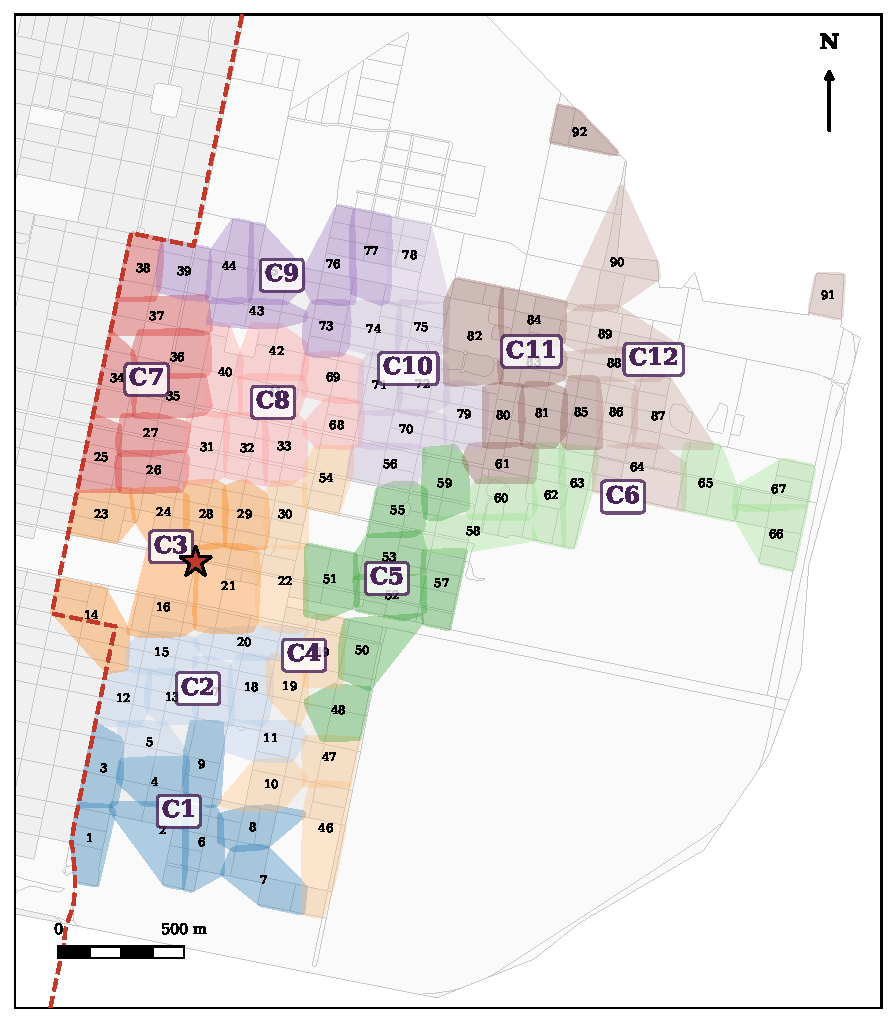
\includegraphics[width=0.95\textwidth]{plano_este_sectores.pdf}
    \caption{Región Este: clusters (C1 a C12) y sectores de diseño (1 a 92).}
    \label{fig:sectores}
\end{figure}

\begin{table}[H]\centering\footnotesize
\caption{Clusters de la Región Este: viviendas, abonados y longitudes.}\label{tab:clusters}
\setlength{\tabcolsep}{3pt}\begin{tabular}{|c|c|r|r|r|r|r|p{3.6cm}|}\hline \textbf{Cluster} & \textbf{Sect.} & \textbf{Viv.} & \textbf{Ab. 1.\textsuperscript{a} et.} & \textbf{Ab. final} & \textbf{L troncal [m]} & \textbf{Cable cl. [m]} & \textbf{Ubicación del CEO} \\ \hline
C1 & 8 & 540 & 243 & 486 & 909 & 1.683 & Avenida Zeballos y Perú \\ \hline
C2 & 8 & 540 & 243 & 486 & 388 & 1.857 & 3 de Febrero y Perú \\ \hline
C3 & 7 & 473 & 213 & 426 & 158 & 1.707 & 9 de Julio y Avenida San Martín \\ \hline
C4 & 8 & 540 & 243 & 486 & 474 & 3.444 & Champagnat y Pasaje Maipú \\ \hline
C5 & 8 & 540 & 243 & 486 & 674 & 2.713 & Boulevard Lardizabal y Garibaldi \\ \hline
C6 & 7 & 473 & 213 & 426 & 1.540 & 2.453 & Los Robles \\ \hline
C7 & 8 & 540 & 243 & 486 & 575 & 1.452 & Leandro N. Alem \\ \hline
C8 & 8 & 540 & 243 & 486 & 581 & 2.113 & Boulevard Hipólito Irigoyen y Justo José de Urquiza \\ \hline
C9 & 7 & 473 & 213 & 426 & 1.302 & 1.542 & 9 de Julio y Avenida Rivadavia \\ \hline
C10 & 8 & 538 & 243 & 485 & 1.317 & 1.811 & Bismark y O'Higgins \\ \hline
C11 & 8 & 517 & 233 & 466 & 1.857 & 2.861 & Avenida Roque Sanz Peña Este y Timoteo Gordillo \\ \hline
C12 & 7 & 439 & 198 & 396 & 2.566 & 2.613 & Hermanas Vicentinas y Pasaje Juan Cruz González Este \\ \hline
\textbf{Total} & \textbf{92} & \textbf{6.153} & \textbf{2.771} & \textbf{5.541} & \multicolumn{3}{l|}{} \\ \hline
\end{tabular}\end{table}


\subsection{Trazas generales}
\label{sec:trazas}
Los cables se tienden en forma aérea sobre la postería, siguiendo los recorridos más cortos por la red de calles. Las longitudes se calcularon sobre el grafo de calles de OpenStreetMap \cite{osm}. Se distinguen tres niveles de cable:

\begin{itemize}
    \item \underline{Troncal o alimentación:} desde el ODF del hub hasta la caja de empalme (CEO) de cada cluster. Cada cluster tiene asignadas 24 fibras, por lo que la capacidad de cada tramo es la suma de los clusters que alimenta. La traza total es de $7{,}22 \, [km]$ (\autoref{fig:troncal} y \autoref{tab:tramos}).
    \item \underline{Cable de cluster:} cable MINI-RA de 24 fibras que parte de la CEO de cluster y recorre las cajas de distribución de sus sectores. En cada caja se abre el tubo y se derivan las fibras del sector sin cortar las que siguen de paso (sangría). Longitud total: $26{,}25 \, [km]$.
    \item \underline{Distribución de sector:} cable MINI-RA de 12 fibras desde la caja de distribución (splitter 1:4) hasta las CTO del sector. Longitud total: $33{,}40 \, [km]$.
    \item \underline{Acometida (drop):} desde la CTO hasta cada vivienda. Su longitud media es de $68 \, [m]$, el 90\,\% de las viviendas queda a menos de $129 \, [m]$ de su CTO y la máxima es de $270 \, [m]$.
\end{itemize}

\begin{figure}[H]
    \centering
    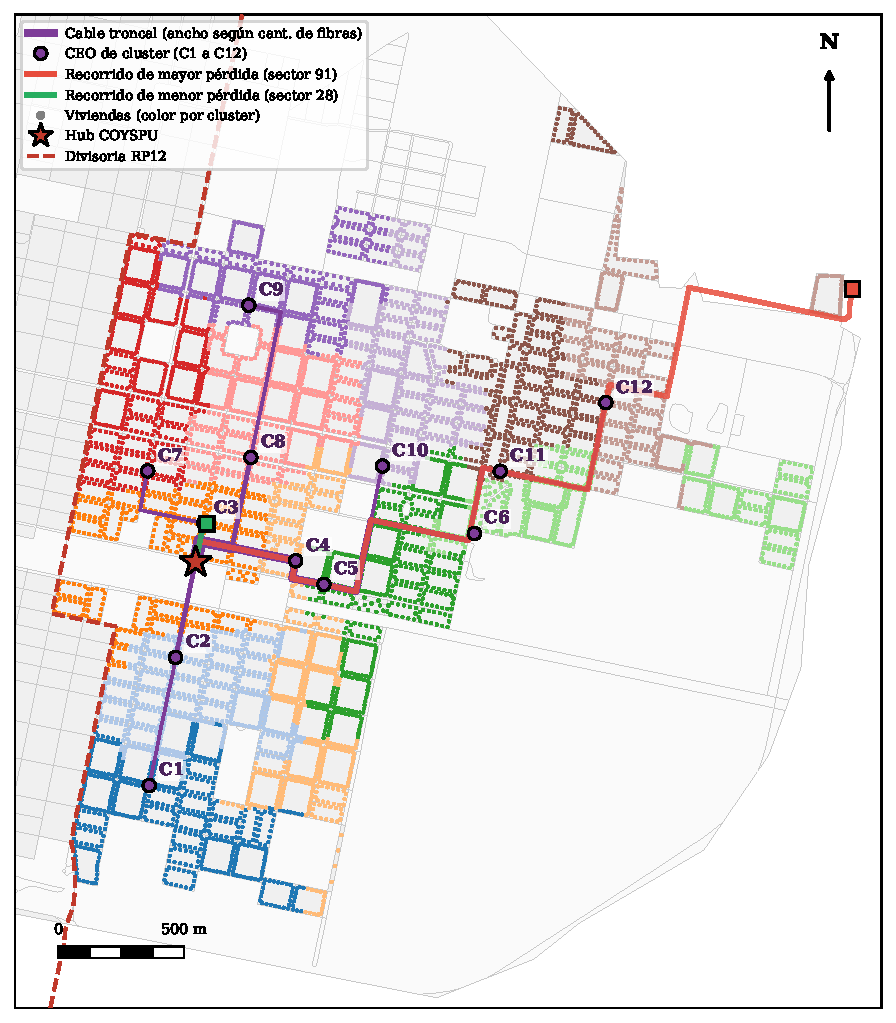
\includegraphics[width=0.95\textwidth]{plano_este_troncal.pdf}
    \caption{Región Este: traza del cable troncal, cajas de empalme de cluster y recorridos de mayor y menor pérdida óptica.}
    \label{fig:troncal}
\end{figure}

\footnotesize\setlength{\tabcolsep}{4pt}\begin{longtable}{|c|l|l|r|r|c|p{4.2cm}|}
\caption{Tramos del cable troncal de la Región Este.}\label{tab:tramos}\\ \hline
\textbf{Tramo} & \textbf{Desde} & \textbf{Hasta} & \textbf{L [m]} & \textbf{Fibras} & \textbf{Cable} & \textbf{Recorrido (calles)} \\ \hline \endfirsthead
\hline \textbf{Tramo} & \textbf{Desde} & \textbf{Hasta} & \textbf{L [m]} & \textbf{Fibras} & \textbf{Cable} & \textbf{Recorrido (calles)} \\ \hline \endhead
CT-01 & Hub COYSPU & D1 & 5 & 240 & 2x144F & 9 de Julio \\ \hline
CT-02 & Hub COYSPU & CEO-C2 & 388 & 48 & 1x48F & 9 de Julio, Perú \\ \hline
CT-03 & D1 & D2 & 128 & 144 & 1x144F & Boulevard Lardizabal \\ \hline
CT-04 & D1 & CEO-C3 & 153 & 72 & 1x72F & 9 de Julio \\ \hline
CT-05 & D1 & CEO-C7 & 569 & 24 & 1x24F & Avenida San Martín, Boulevard Lardizabal, Italia \\ \hline
CT-06 & D2 & CEO-C4 & 340 & 48 & 1x48F & Justo José de Urquiza, Pasaje Maipú \\ \hline
CT-07 & D2 & CEO-C5 & 398 & 96 & 1x96F & Boulevard Lardizabal, Jujuy \\ \hline
CT-08 & CEO-C3 & D3 & 144 & 48 & 1x48F & 9 de Julio \\ \hline
CT-09 & D3 & CEO-C8 & 277 & 24 & 1x24F & Avenida Belgrano, Justo José de Urquiza \\ \hline
CT-10 & D3 & CEO-C9 & 851 & 24 & 1x24F & 9 de Julio \\ \hline
CT-11 & CEO-C2 & CEO-C1 & 521 & 24 & 1x24F & Perú \\ \hline
CT-12 & CEO-C4 & CEO-C10 & 695 & 24 & 1x24F & Avenida Belgrano, Bismark, Boulevard Hipólito Irigoyen \\ \hline
CT-13 & CEO-C5 & D4 & 270 & 72 & 1x72F & Avenida San Martín, Garibaldi \\ \hline
CT-14 & D4 & CEO-C6 & 590 & 48 & 1x48F & Avenida San Martín, Fuerza Aérea Argentina, Los Robles \\ \hline
CT-15 & D4 & CEO-C11 & 898 & 24 & 1x24F & Avenida Roque Sanz Peña Este, Bismark, Boulevard Roque Sáenz Peña \\ \hline
CT-16 & CEO-C6 & CEO-C12 & 994 & 24 & 1x24F & Avenida Belgrano, Avenida Roque Sanz Peña Este, Hermanas Vicentinas \\ \hline
\multicolumn{3}{|r|}{\textbf{Total de traza}} & \textbf{7.222} & \multicolumn{3}{l|}{} \\ \hline
\end{longtable}

\begin{table}[H]\centering\footnotesize
\caption{Ubicación de las cajas de empalme del troncal.}\label{tab:nodos}
\begin{tabular}{|l|l|}\hline \textbf{Identificación} & \textbf{Ubicación (intersección de calles)} \\ \hline
Hub COYSPU & 9 de Julio 99 (Cooperativa COYSPU) \\ \hline
CEO-C1 & Avenida Zeballos y Perú \\ \hline
CEO-C2 & 3 de Febrero y Perú \\ \hline
CEO-C3 & 9 de Julio y Avenida San Martín \\ \hline
CEO-C4 & Champagnat y Pasaje Maipú \\ \hline
CEO-C5 & Boulevard Lardizabal y Garibaldi \\ \hline
CEO-C6 & Los Robles \\ \hline
CEO-C7 & Leandro N. Alem \\ \hline
CEO-C8 & Boulevard Hipólito Irigoyen y Justo José de Urquiza \\ \hline
CEO-C9 & 9 de Julio y Avenida Rivadavia \\ \hline
CEO-C10 & Bismark y O'Higgins \\ \hline
CEO-C11 & Avenida Roque Sanz Peña Este y Timoteo Gordillo \\ \hline
CEO-C12 & Hermanas Vicentinas y Pasaje Juan Cruz González Este \\ \hline
D1 & 9 de Julio y Boulevard Lardizabal \\ \hline
D2 & Boulevard Lardizabal y Justo José de Urquiza \\ \hline
D3 & 9 de Julio y Avenida Belgrano \\ \hline
D4 & Avenida San Martín y Bismark \\ \hline
\end{tabular}\end{table}


\textbf{Ubicación de cajas y splitters:}
\begin{itemize}
    \item \underline{Cajas de empalme del troncal (FK-CEO-4M):} en las 12 CEO de cluster y en los 4 puntos de derivación D1 a D4 (\autoref{tab:nodos}), donde cambia la capacidad del cable.
    \item \underline{Cajas de distribución (FK-CEO-4M con splitter 1:4):} una por sector (92 en total), en la esquina que minimiza el recorrido de distribución hasta sus CTO. Su ubicación se lista en el \autoref{anexo:sectores}.
    \item \underline{Cajas terminales (FK-CTO-16MC con splitter 1:16):} 365 cajas en postes de esquina, cada una para hasta 17 viviendas.
\end{itemize}

\textbf{Reservas de cable:} se deja un rulo de reserva de $20 \, [m]$ en cada CEO y caja de distribución y de $10 \, [m]$ en cada CTO. Esto permite reabrir los empalmes y reubicar las cajas sin reemplazar el cable. Además, se adiciona un 10\,\% a las longitudes de traza por catenaria, bajadas y desvíos en los postes.

\subsubsection{Aspectos que requieren verificación de campo}
\label{sec:verificacion}
\begin{itemize}
    \item \underline{Postería:} propiedad, estado, altura y vanos reales, y acuerdo de uso con su propietario (la COYSPU no figura como distribuidora eléctrica \cite{coyspu}, por lo que el permiso debe gestionarse con la distribuidora o el municipio).
    \item \underline{Cruces especiales:} cruces de la RN9, de la RP12 y de la traza ferroviaria, que pueden requerir tendido subterráneo o permisos de Vialidad y del concesionario ferroviario.
    \item \underline{Viviendas reales:} cantidad de viviendas por manzana, en especial en el centro, donde los edificios de departamentos requieren un diseño vertical propio, y en los barrios en expansión de la periferia, donde OpenStreetMap puede no estar actualizado.
    \item \underline{Calles sin nombre y loteos nuevos} en el noreste de la región (sectores 91 y 92).
    \item \underline{Ubicación exacta del nodo REFEFO} y de la red de fibra existente de la COYSPU, que podría reutilizarse para el enlace mayorista.
\end{itemize}

\subsection{Desarrollo de dos sectores}
\label{sec:sectores}
Se desarrollan en detalle dos sectores representativos:
\begin{itemize}
    \item El \textbf{sector 28} (cluster C3), en el centro, junto al hub, que contiene el recorrido de menor pérdida de la región.
    \item El \textbf{sector 90} (cluster C12), en la periferia noreste: es el sector completo, con 4 CTO, más alejado del hub.
\end{itemize}

En ambos casos las fibras del cable de distribución de 12 fibras se asignan así:
\begin{itemize}
    \item F1 a F4: salidas 1 a 4 del splitter 1:4, una para cada CTO.
    \item F5 a F8: crecimiento.
    \item F9 a F12: reserva.
\end{itemize}
En cada CTO, el splitter 1:16 conectorizado tiene sus salidas numeradas del 1 al 16, y cada salida corresponde a una vivienda.

\subsubsection{Sector 28}
El sector 28 tiene 67 viviendas en las manzanas comprendidas entre 9 de Julio, Av. San Martín, Av. Belgrano y Pasaje Maipú (\autoref{fig:sector28}). Su caja de distribución CD-28 está en 9 de Julio y Av. San Martín, en el mismo poste que la CEO del cluster C3, por lo que ambas funciones pueden resolverse en una única caja FK-CEO-4M. El cable de distribución mide $230 \, [m]$ y la acometida más larga es de $109 \, [m]$ (\autoref{tab:sector28}).

\begin{figure}[H]
    \centering
    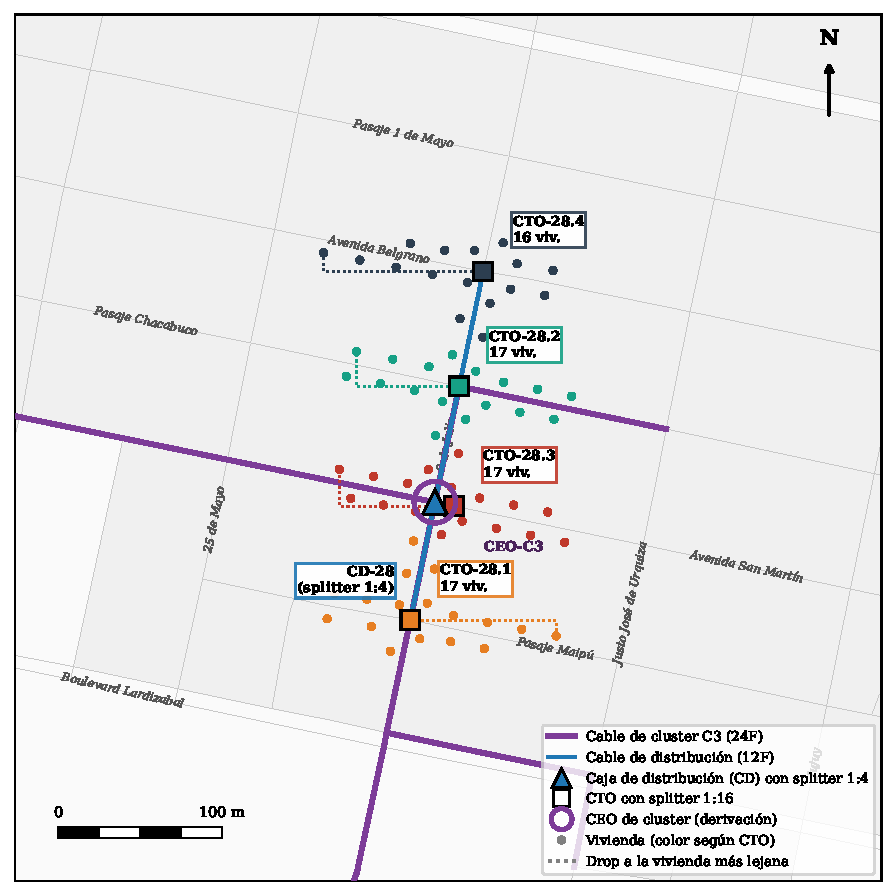
\includegraphics[width=0.85\textwidth]{plano_sector_28.pdf}
    \caption{Plano ampliado del sector 28 (cluster C3).}
    \label{fig:sector28}
\end{figure}

\begin{table}[H]\centering\footnotesize
\caption{Cajas terminales del sector 28 (cluster C3).}\label{tab:sector28}
\begin{tabular}{|c|p{4.0cm}|r|r|r|c|}\hline \textbf{CTO} & \textbf{Ubicación} & \textbf{Viv.} & \textbf{Desde CD [m]} & \textbf{Drop máx. [m]} & \textbf{Fibra/salida} \\ \hline
CTO-28.1 & 9 de Julio y Pasaje Maipú & 17 & 74 & 99 & F1 / 1 \\ \hline
CTO-28.2 & 9 de Julio y Pasaje Chacabuco & 17 & 72 & 84 & F2 / 2 \\ \hline
CTO-28.3 & Avenida San Martín & 17 & 12 & 93 & F3 / 3 \\ \hline
CTO-28.4 & 9 de Julio y Avenida Belgrano & 16 & 144 & 109 & F4 / 4 \\ \hline
\end{tabular}\end{table}


\subsubsection{Sector 90}
El sector 90 tiene 67 viviendas en el noreste de la región, alrededor de Hermanas Vicentinas y Soberanía Nacional Este (\autoref{fig:sector90}). Su caja de distribución CD-90 está en Hermanas Vicentinas y Soberanía Nacional Este, a $2{,}92 \, [km]$ del hub por el troncal y el cable de cluster. Por la menor densidad de viviendas, el cable de distribución es más largo ($633 \, [m]$) y la acometida más larga alcanza $227 \, [m]$ (\autoref{tab:sector90}). Es aceptable para un drop autosoportado, pero la ubicación de la CTO-90.4 debe revisarse en campo para acortarla.

\begin{figure}[H]
    \centering
    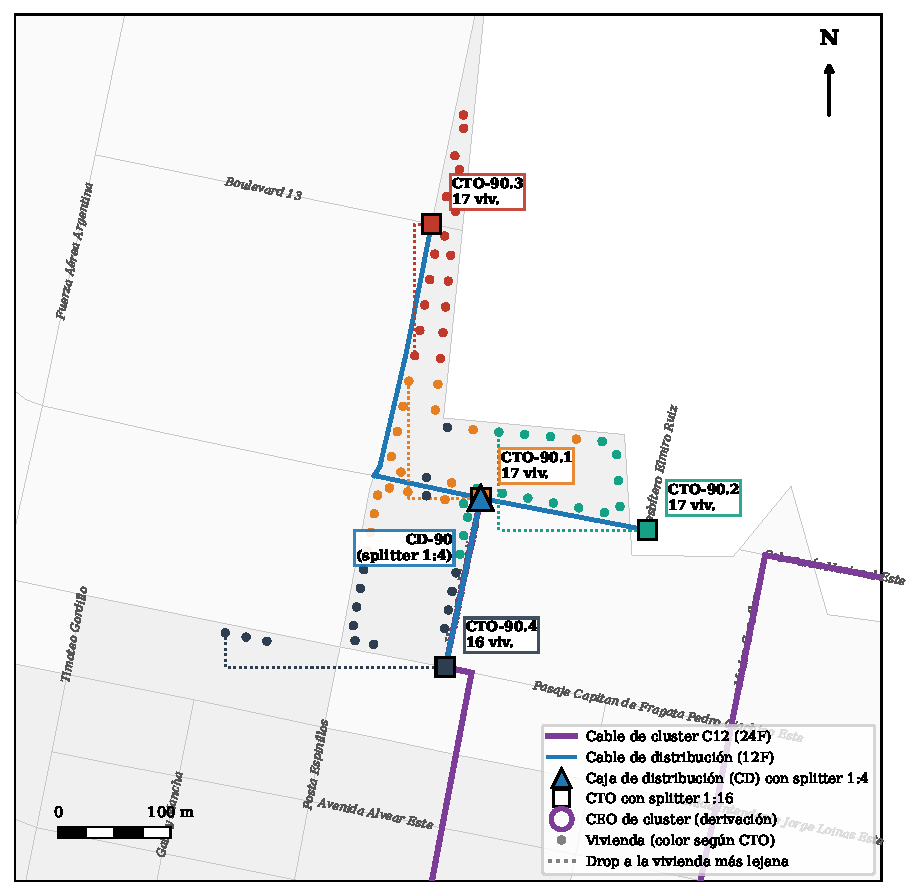
\includegraphics[width=0.85\textwidth]{plano_sector_90.pdf}
    \caption{Plano ampliado del sector 90 (cluster C12).}
    \label{fig:sector90}
\end{figure}

\begin{table}[H]\centering\footnotesize
\caption{Cajas terminales del sector 90 (cluster C12).}\label{tab:sector90}
\begin{tabular}{|c|p{4.0cm}|r|r|r|c|}\hline \textbf{CTO} & \textbf{Ubicación} & \textbf{Viv.} & \textbf{Desde CD [m]} & \textbf{Drop máx. [m]} & \textbf{Fibra/salida} \\ \hline
CTO-90.1 & Hermanas Vicentinas y Soberanía Nacional Este & 17 & 0 & 169 & F1 / 1 \\ \hline
CTO-90.2 & Presbítero Elmiro Ruiz y Soberanía Nacional Este & 17 & 151 & 220 & F2 / 2 \\ \hline
CTO-90.3 & Boulevard 13 y Posta Espinillos & 17 & 328 & 132 & F3 / 3 \\ \hline
CTO-90.4 & Hermanas Vicentinas y Pasaje Capitan de Fragata Pedro Giachino Este & 16 & 154 & 227 & F4 / 4 \\ \hline
\end{tabular}\end{table}


\pendiente{Región Oeste: organización en clusters y sectores, trazas y desarrollo de sus dos sectores, a cargo de Mendes Rosa y Monja.}

\newpage


\section{Dimensionamiento de fibras y capacidad}
\label{sec:dimensionamiento}

\subsection{Fibras y cables}
\label{sec:fibras}
% Consigna 6.1: fibras necesarias en cada tramo para la cobertura final. Diferenciar:
% primera etapa, crecimiento, reserva y otras aplicaciones.
% Seleccionar capacidades comerciales de cable y presentar una tabla por tramo con
% longitud, cantidad de fibras y asignación.
\pendiente{tabla por tramo: longitud, fibras y asignación (uso, crecimiento, reserva).}

\subsection{Puertos GPON y ancho de banda}
\label{sec:puertos}
% Consigna 6.2: definir y justificar:
% - Máximo de abonados por puerto GPON.
% - Relación de división total y etapas de división.
% - Puertos necesarios en la primera etapa y en la cobertura final.
% - Capacidad compartida y demanda estimada en hora pico.
% - Criterio de simultaneidad o sobrecontratación.
% Distinguir la relación de división óptica del criterio de sobrecontratación y explicar
% cómo ambos condicionan la capacidad ofrecida.
\pendiente{abonados por puerto, relación de división, cantidad de puertos y demanda en hora pico.}

\newpage


\section{Conectividad mayorista}
\label{sec:mayorista}

\subsection{Punto de interconexión y tecnología}
Marcos Juárez cuenta con un nodo activo de la Red Federal de Fibra Óptica, según el listado de puntos de conexión de ARSAT de febrero de 2026 \cite{arsat_nodos}. Se propone conectar el hub de la COYSPU a ese nodo como proveedor mayorista de tránsito IP. La ubicación exacta del nodo no se publica, por lo que se adopta como \textbf{supuesto de diseño} que se encuentra dentro del ejido urbano, a no más de $4 \, [km]$ de recorrido del hub. Debe verificarse con ARSAT al momento de contratar el servicio.

\begin{itemize}
    \item \underline{Tecnología del enlace:} enlace punto a punto de fibra óptica con interfaces Ethernet de $10 \, [Gbps]$ (10GBASE-LR, $1310 \, [nm]$). Se dimensiona con la misma metodología que el enlace de la Parte 1 \cite{informe_p1}.
    \item \underline{Recorrido:} cable aéreo CFOA-SM-AS80-S TS de 24 fibras desde el hub hasta el nodo REFEFO. Si la ubicación del nodo lo permite, puede aprovecharse la red de fibra existente de la cooperativa, que cuenta con un anillo de cuatro nodos en la ciudad \cite{coyspu}. Las fibras restantes quedan para un segundo vínculo redundante o para otros servicios.
    \item \underline{Equipos:} en el hub, un router de borde con funciones de BNG (autenticación y gestión de sesiones de los abonados) y un switch de agregación al que se conectan las 6 OLT de la Región Este, cada una con dos enlaces de $10 \, [GE]$ en agregación (LAG). La OLT V1600G2-B dispone de cuatro puertos SFP+ de $10 \, [GE]$ de subida \cite{vsol_olt}. Se recomienda incorporar en el hub cachés de contenido de los principales proveedores, que sirven localmente parte del tráfico y reducen la capacidad mayorista necesaria.
\end{itemize}

\textbf{Verificación del enlace:} con módulos SFP+ 10GBASE-LR (Tx de $-8{,}2$ a $+0{,}5 \, [dBm]$; sensibilidad $< -14{,}4 \, [dBm]$) \cite{fs_10glr}, el presupuesto óptico es de $6{,}2 \, [dB]$. Reservando $3 \, [dB]$ de margen de seguridad y descontando cuatro conectores ($1{,}2 \, [dB]$) y dos empalmes ($0{,}2 \, [dB]$), quedan $1{,}8 \, [dB]$ para la fibra. Con $0{,}38 \, [dB/km]$, el enlace admite hasta $4{,}7 \, [km]$, lo que cubre la distancia supuesta. Si el nodo estuviera más lejos, se reemplazarían los módulos por 10GBASE-ER ($40 \, [km]$).

\subsection{Ancho de banda requerido}
El enlace mayorista es compartido por las dos regiones, por lo que se dimensiona para la red completa. Para la Región Oeste se usa la estimación de este informe, a confirmar por el otro equipo. Se aplica la demanda en la hora de mayor tráfico de $5 \, [Mbps]$ por abonado (\autoref{eq:demanda}) y un margen de crecimiento del 30\,\%:

\begin{table}[H]
    \centering
    \caption{Ancho de banda mayorista requerido (bajada).}
    \label{tab:mayorista}
    \begin{tabular}{|l|r|r|}
        \hline
        \textbf{Concepto} & \textbf{Primera etapa} & \textbf{Cobertura final} \\
        \hline
        Abonados Región Este & $2.771$ & $5.541$ \\
        Abonados Región Oeste (estimado) & $2.692$ & $5.384$ \\
        Total de abonados & $5.463$ & $10.925$ \\
        Demanda en hora pico ($\times 5 \, [Mbps]$) & $27{,}3 \, [Gbps]$ & $54{,}6 \, [Gbps]$ \\
        Con margen de crecimiento del 30\,\% & $35{,}5 \, [Gbps]$ & $71{,}0 \, [Gbps]$ \\
        \hline
        \textbf{Capacidad a contratar} & $4 \times 10 \, [Gbps]$ & $100 \, [Gbps]$ \\
        \hline
    \end{tabular}
\end{table}

Para la primera etapa se propone contratar \textbf{$40 \, [Gbps]$ como cuatro enlaces de $10 \, [Gbps]$ en LAG}, sobre dos pares de fibras, o mediante multiplexación CWDM sobre un par. En la cobertura final la demanda requiere migrar a una interfaz de $100 \, [Gbps]$ o ampliar el LAG. El tráfico que resuelvan las cachés locales reduce estas cifras. Si la televisión se brinda sobre IP, debe sumarse su tráfico (\autoref{sec:television}).

\subsection{Capacidad mayorista frente a capacidad de los puertos GPON}
La suma de la capacidad de los puertos GPON de la Región Este es de $92 \times 2{,}488 \approx 229 \, [Gbps]$, muy superior al ancho de banda mayorista requerido. No hay contradicción:
\begin{itemize}
    \item La capacidad de un puerto GPON se comparte solo entre los abonados de su sector (hasta 61). Debe alcanzar para la demanda simultánea de ese grupo y para las ráfagas de un abonado que use su plan completo.
    \item La capacidad mayorista agrega el tráfico de todos los abonados de la red. Como no todos los sectores tienen su pico al mismo tiempo ni todos los abonados están activos, se dimensiona con la demanda promedio en la hora pico (multiplexación estadística).
\end{itemize}
En consecuencia, el cuello de botella de la red en la hora pico no son los puertos GPON (12\,\% de ocupación), sino el enlace mayorista, que es además el costo recurrente más importante del operador.

\newpage


\section{Presupuesto óptico}
\label{sec:presupuesto}
% Consigna 8: sentido descendente (OLT -> ONT, 1490 nm) y ascendente (ONT -> OLT, 1310 nm),
% con las especificaciones de los equipos seleccionados. Incluir:
% - Potencias mínima y máxima de transmisión.
% - Sensibilidad y nivel máximo admisible de los receptores.
% - Atenuación de la fibra para cada longitud de onda.
% - Pérdidas de splitters, conectores y empalmes.
% - Margen de ingeniería (envejecimiento, reparaciones, incertidumbres).
% Verificar en ambos sentidos:
% 1. Recorrido de MAYOR pérdida -> potencia recibida suficiente.
% 2. Recorrido de MENOR pérdida -> no superar el nivel máximo del receptor.
% Identificar estos recorridos en el plano, presentar tablas y proponer correcciones si algo no cumple.
% Se puede reutilizar la metodología y el formato de tablas de la Parte 1 (Parte_1/parteB.tex).

\subsection{Parámetros de los equipos y de la ODN}
\label{sec:parametros_presupuesto}
\pendiente{potencias, sensibilidades y pérdidas unitarias por longitud de onda.}

\subsection{Sentido descendente (OLT $\rightarrow$ ONT)}
\label{sec:descendente}
\pendiente{recorridos de mayor y menor pérdida en sentido descendente.}

\subsection{Sentido ascendente (ONT $\rightarrow$ OLT)}
\label{sec:ascendente}
\pendiente{recorridos de mayor y menor pérdida en sentido ascendente.}

\newpage


\section{Diagramas de cableado y asignación de fibras}
\label{sec:cableado}
% Consigna 9: diagramas para seguir la continuidad óptica desde la OLT hasta las terminales de abonado.
% - Diferenciar tramos de alimentación/troncal, distribución y acceso al abonado.
% - Si se usan los términos dispersión, drop y acometida, definir el alcance de cada uno.
% - Identificar cables, fibras, cajas, empalmes, splitters y puertos de salida,
%   con correspondencia con los planos.
\pendiente{diagramas de continuidad óptica y asignación de fibras.}

\newpage


\section{Alternativas para distribuir televisión}
\label{sec:television}

\subsection{Televisión sobre IP}
\label{sec:iptv}
% Diferenciar distribución multicast y unicast; efecto sobre la capacidad GPON y la conectividad mayorista.
\pendiente{IPTV multicast vs. unicast y su efecto en GPON y en el enlace mayorista.}

\subsection{Video overlay óptico}
\label{sec:overlay}
% Equipos y componentes adicionales (transmisor de video a 1550 nm, EDFA, WDM), compatibilidad con la ODN
% y necesidad de un presupuesto óptico específico.
\pendiente{video overlay a 1550 nm: equipos, compatibilidad y presupuesto óptico.}

\subsection{Comparación y elección}
\label{sec:tv_eleccion}
% Qué tráfico genera cada alternativa, por dónde circula, qué recursos usa.
% Justificar cuál se elige para el proyecto y bajo qué condiciones.
\pendiente{comparación de ambas alternativas y elección justificada.}

\newpage


\section{Conclusiones y limitaciones del diseño}
\label{sec:conclusiones}
% La consigna pide explícitamente conclusiones Y limitaciones del diseño
% (supuestos no verificados, puntos que requieren verificación de campo, etc.).
\pendiente{conclusiones y limitaciones del diseño.}

\newpage


\nocite{*}
\printbibliography[heading=bibintoc, title={Bibliografía y Referencias}]

\newpage
\appendix
\section{Sectores de diseño de la Región Este}
\label{anexo:sectores}
La tabla lista los 92 sectores de la Región Este:
\begin{itemize}
    \item Cluster al que pertenece cada sector.
    \item Viviendas que atiende y cantidad de cajas terminales.
    \item Ubicación de su caja de distribución.
    \item Longitud de red desde el hub: troncal más cable de cluster.
    \item Longitud del cable de distribución.
    \item Acometida más larga del sector.
\end{itemize}
Los datos y los planos se generan con los scripts de la carpeta \texttt{diseno/} del repositorio, a partir de la cartografía de OpenStreetMap \cite{osm}.

\footnotesize\setlength{\tabcolsep}{4pt}\begin{longtable}{|c|c|r|c|p{4.2cm}|r|r|r|}
\caption{Sectores de diseño de la Región Este.}\label{tab:sectores}\\ \hline
\textbf{Sect.} & \textbf{Clúst.} & \textbf{Viv.} & \textbf{CTO} & \textbf{Caja de distribución (CD)} & \textbf{Red [m]} & \textbf{Distr. [m]} & \textbf{Drop [m]} \\ \hline \endfirsthead
\hline \textbf{Sect.} & \textbf{Clúst.} & \textbf{Viv.} & \textbf{CTO} & \textbf{Caja de distribución (CD)} & \textbf{Red [m]} & \textbf{Distr. [m]} & \textbf{Drop [m]} \\ \hline \endhead
1 & C1 & 68 & 4 & Avenida Pueyrredón y Uruguay & 1.328 & 442 & 128 \\ \hline
2 & C1 & 67 & 4 & Avenida Saavedra y Venezuela & 1.184 & 375 & 160 \\ \hline
3 & C1 & 67 & 4 & Avenida Zeballos y Uruguay & 1.039 & 403 & 238 \\ \hline
4 & C1 & 68 & 4 & Avenida Zeballos y Perú & 909 & 331 & 199 \\ \hline
5 & C2 & 67 & 4 & Avenida Quintana y Perú & 763 & 338 & 187 \\ \hline
6 & C1 & 67 & 4 & Avenida Saavedra y Ecuador & 1.315 & 225 & 134 \\ \hline
7 & C1 & 68 & 4 & Avenida Pueyrredón y Chile & 1.712 & 372 & 165 \\ \hline
8 & C1 & 67 & 4 & Avenida Saavedra y Pasaje Malvinas Argentinas & 1.509 & 410 & 111 \\ \hline
9 & C1 & 68 & 4 & Pasaje Ingeniero Carlos Cagnolo y Venezuela & 1.109 & 498 & 146 \\ \hline
10 & C4 & 68 & 4 & Avenida Zeballos y Pasaje Malvinas Argentinas & 1.531 & 419 & 190 \\ \hline
11 & C2 & 67 & 4 & Avenida San Juan y Chile & 1.123 & 412 & 168 \\ \hline
12 & C2 & 68 & 4 & Avenida San Juan y Uruguay & 734 & 277 & 208 \\ \hline
13 & C2 & 67 & 4 & 24 de Septiembre y Perú & 535 & 277 & 189 \\ \hline
14 & C3 & 68 & 4 & Avenida Carlos Pellegrini y General Roca & 1.017 & 614 & 187 \\ \hline
15 & C2 & 68 & 4 & 3 de Febrero y Perú & 388 & 271 & 155 \\ \hline
16 & C3 & 67 & 4 & Boulevard Juan B. Justo y Uruguay & 618 & 383 & 228 \\ \hline
17 & C2 & 67 & 4 & 24 de Septiembre y Venezuela & 661 & 346 & 130 \\ \hline
18 & C2 & 68 & 4 & Avenida Mendoza y Ecuador & 716 & 275 & 149 \\ \hline
19 & C4 & 67 & 4 & Avenida Mendoza y Brasil & 1.021 & 405 & 132 \\ \hline
20 & C2 & 68 & 4 & Cochabamba y Ecuador & 790 & 404 & 156 \\ \hline
21 & C3 & 68 & 4 & Justo José de Urquiza & 488 & 531 & 202 \\ \hline
22 & C4 & 67 & 4 & Champagnat y Pasaje Maipú & 474 & 349 & 139 \\ \hline
23 & C3 & 68 & 4 & Francisco Beiró y Pasaje Maipú & 620 & 293 & 155 \\ \hline
24 & C3 & 67 & 4 & 25 de Mayo y Avenida San Martín & 288 & 461 & 106 \\ \hline
25 & C7 & 67 & 4 & Pasaje 1 de Mayo & 846 & 273 & 151 \\ \hline
26 & C7 & 68 & 4 & Leandro N. Alem & 575 & 255 & 147 \\ \hline
27 & C7 & 67 & 4 & Boulevard Hipólito Irigoyen y Leandro N. Alem & 712 & 214 & 150 \\ \hline
28 & C3 & 67 & 4 & 9 de Julio y Avenida San Martín & 158 & 230 & 109 \\ \hline
29 & C3 & 68 & 4 & Justo José de Urquiza y Pasaje Chacabuco & 360 & 299 & 142 \\ \hline
30 & C4 & 67 & 4 & Jujuy y Pasaje Chacabuco & 748 & 458 & 141 \\ \hline
31 & C8 & 68 & 4 & 25 de Mayo y Boulevard Hipólito Irigoyen & 840 & 400 & 188 \\ \hline
32 & C8 & 68 & 4 & Boulevard Hipólito Irigoyen y Justo José de Urquiza & 581 & 228 & 191 \\ \hline
33 & C8 & 67 & 4 & Jujuy y O'Higgins & 789 & 173 & 158 \\ \hline
34 & C7 & 67 & 4 & Francisco Beiró y Pasaje Bonetto & 1.069 & 486 & 119 \\ \hline
35 & C7 & 68 & 4 & Boulevard Roque Sáenz Peña y Leandro N. Alem & 879 & 146 & 195 \\ \hline
36 & C7 & 67 & 4 & Avenida Avellaneda y Leandro N. Alem & 1.021 & 325 & 183 \\ \hline
37 & C7 & 68 & 4 & Avenida Santa Fe y Francisco Beiró & 1.286 & 266 & 228 \\ \hline
38 & C7 & 68 & 4 & Avenida Alvear y Francisco Beiró & 1.571 & 534 & 196 \\ \hline
39 & C9 & 67 & 4 & Avenida Alvear y Leandro N. Alem & 1.703 & 288 & 159 \\ \hline
40 & C8 & 67 & 4 & 9 de Julio y Avenida Avellaneda & 1.013 & 412 & 188 \\ \hline
41 & C8 & 68 & 4 & Avenida Avellaneda y Jujuy & 1.012 & 400 & 216 \\ \hline
42 & C8 & 67 & 4 & Avenida Santa Fe y Justo José de Urquiza & 1.028 & 245 & 175 \\ \hline
43 & C9 & 68 & 4 & 9 de Julio y Avenida Rivadavia & 1.302 & 338 & 153 \\ \hline
44 & C9 & 68 & 4 & 25 de Mayo y Avenida Alvear & 1.572 & 321 & 209 \\ \hline
45 & C9 & 67 & 4 & 9 de Julio y Avenida Alvear & 1.443 & 303 & 153 \\ \hline
46 & C4 & 68 & 4 & Avenida Zeballos y Rafael Núñez & 1.721 & 543 & 190 \\ \hline
47 & C4 & 67 & 4 & Avenida San Juan y Dean Funes & 1.553 & 437 & 217 \\ \hline
48 & C5 & 67 & 4 & Avenida Mendoza y Dean Funes & 1.666 & 288 & 234 \\ \hline
49 & C4 & 68 & 4 & Boulevard Juan B. Justo y Chile & 861 & 424 & 197 \\ \hline
50 & C5 & 67 & 4 & Boulevard Juan B. Justo y Dean Funes & 1.377 & 499 & 168 \\ \hline
51 & C5 & 67 & 4 & Boulevard Lardizabal y Garibaldi & 674 & 217 & 173 \\ \hline
52 & C5 & 68 & 4 & Boulevard Lardizabal y Juan José Paso & 935 & 224 & 152 \\ \hline
53 & C5 & 67 & 4 & Avenida San Martín y Juan José Paso & 1.074 & 276 & 232 \\ \hline
54 & C4 & 68 & 4 & Champagnat y Pasaje 1 de Mayo & 763 & 302 & 163 \\ \hline
55 & C5 & 68 & 4 & Juan José Paso y Pasaje 1 de Mayo & 1.274 & 275 & 140 \\ \hline
56 & C10 & 67 & 4 & Bismark y O'Higgins & 1.317 & 353 & 176 \\ \hline
57 & C5 & 68 & 4 & Fuerza Aérea Argentina y Pasaje Maipú & 1.268 & 433 & 165 \\ \hline
58 & C6 & 67 & 4 & Los Robles & 1.540 & 403 & 151 \\ \hline
59 & C5 & 68 & 4 & Boulevard Hipólito Irigoyen y Independencia & 1.488 & 171 & 171 \\ \hline
60 & C6 & 68 & 4 & Los Almendros y Los Álamos & 1.799 & 664 & 106 \\ \hline
61 & C11 & 67 & 4 & Avenida Roque Sanz Peña Este y Timoteo Gordillo & 1.857 & 338 & 120 \\ \hline
62 & C6 & 67 & 4 & Posta Espinillos & 1.996 & 653 & 157 \\ \hline
63 & C6 & 68 & 4 & Avenida Roque Sanz Peña Este y Posta Espinillos & 2.102 & 400 & 190 \\ \hline
64 & C12 & 67 & 4 & Avenida Avellaneda Este y Madre González & 3.023 & 306 & 270 \\ \hline
65 & C6 & 68 & 4 & Avenida Avellaneda Este y Calle Nº 20 & 2.793 & 247 & 213 \\ \hline
66 & C6 & 68 & 4 & Avenida Roque Sanz Peña Este y Calle Nº 22 & 2.906 & 321 & 182 \\ \hline
67 & C6 & 67 & 4 & Avenida Avellaneda Este y Calle Nº 22 & 3.037 & 361 & 151 \\ \hline
68 & C8 & 68 & 4 & Boulevard Roque Sáenz Peña y Garibaldi & 1.131 & 340 & 142 \\ \hline
69 & C8 & 67 & 4 & Champagnat y Pasaje Parque & 1.215 & 276 & 239 \\ \hline
70 & C10 & 67 & 4 & Bismark y Pasaje Bonetto & 1.473 & 399 & 149 \\ \hline
71 & C10 & 68 & 4 & Bismark y Pasaje Parque & 1.617 & 407 & 212 \\ \hline
72 & C10 & 67 & 4 & Avenida Santa Fe y Juan José Paso & 1.815 & 378 & 154 \\ \hline
73 & C9 & 67 & 4 & Avenida Rivadavia y Jujuy & 1.564 & 328 & 175 \\ \hline
74 & C10 & 68 & 4 & Avenida Rivadavia y Garibaldi & 1.966 & 266 & 190 \\ \hline
75 & C10 & 67 & 4 & Avenida Rivadavia & 1.875 & 311 & 106 \\ \hline
76 & C9 & 68 & 4 & Avenida Intendente Jorge Loinas y Jujuy & 1.750 & 446 & 146 \\ \hline
77 & C9 & 68 & 4 & 2 de Abril y Soldado Mario Almonacid & 2.041 & 628 & 171 \\ \hline
78 & C10 & 67 & 4 & 8 de Setiembre y Soldado Mario Almonacid & 2.280 & 482 & 145 \\ \hline
79 & C10 & 67 & 4 & Avenida Avellaneda y Independencia & 1.801 & 218 & 128 \\ \hline
80 & C11 & 68 & 4 & Avenida Santa Fe Este y Fuerza Aérea Argentina & 2.207 & 374 & 118 \\ \hline
81 & C11 & 67 & 4 & Avenida Santa Fe Este y Gato y Mancha & 2.248 & 218 & 158 \\ \hline
82 & C11 & 68 & 4 & Avenida Rivadavia y Calle Sin Nombre & 2.524 & 854 & 229 \\ \hline
83 & C11 & 68 & 4 & Avenida Rivadavia Este y Timoteo Gordillo & 2.282 & 259 & 132 \\ \hline
84 & C11 & 67 & 4 & Avenida Intendente Jorge Loinas Este y Timoteo Gordillo & 2.495 & 451 & 150 \\ \hline
85 & C11 & 67 & 4 & Avenida Santa Fe Este y Posta Espinillos & 2.366 & 267 & 144 \\ \hline
86 & C12 & 68 & 4 & Hermanas Vicentinas y Pasaje Juan Cruz González Este & 2.566 & 391 & 113 \\ \hline
87 & C12 & 67 & 4 & Madre González y Pasaje Juan Cruz González Este & 2.801 & 360 & 149 \\ \hline
88 & C12 & 68 & 4 & Hermanas Vicentinas y Pasaje Paul Harris Este & 2.713 & 442 & 197 \\ \hline
89 & C12 & 68 & 4 & Avenida Intendente Jorge Loinas Este y Hermanas Vicentinas & 2.851 & 429 & 202 \\ \hline
90 & C12 & 67 & 4 & Hermanas Vicentinas y Soberanía Nacional Este & 3.103 & 633 & 227 \\ \hline
91 & C12 & 34 & 2 & sin nombre & 4.024 & 72 & 183 \\ \hline
92 & C11 & 45 & 3 & Maestra Pola Liendo y Timoteo Gordillo & 3.458 & 327 & 131 \\ \hline
\end{longtable}


\end{document}
